\chapter{Near Detector Beamline Measurements (WBS 130.03.03)}
\label{ch:nd-blm}

\fixme{Starting from the fall 2012 CDR content}

\section{Introduction}
\label{sec:nd-blm-intro}

This chapter defines the DUNE strategy for measurements of secondary
beam particles in the region behind the beam absorber. 
Those measurements are designed to provide constraints 
on the neutrino flux at the near and far
detectors, and data on the pulse-to-pulse variation
of the beam for beam diagnostic purposes. A description of equipment
for monitoring the proton beam's interaction with the proton target
can be found in Volume 2: The Beamline at the Near Site. 

The measurements and apparatus described in this chapter fall into
the catagory of equipment designed specifically for DUNE to
detect muons exiting the decay tunnel. 

\section{Design Considerations}
\label{sec:nd-blm-design}

\subsection{General}
The requirements for the beamline measurements, 
as discussed in the NDC requirements documentation~\cite{nd_requirements_doc}, are intimately related to how well the neutrino flux must be known.
Given that DUNE does not have the luxury to construct identical Near and Far Detectors, 
a near-far comparison is more complicated than it was in
the MINOS experiment~\cite{gnumi-validation}, for example.   
While external hadron-production measurements can place strong constraints on the pion and kaon production in the target,
they do not provide any confirmation of the simulation of other key features, such as the horn focusing, secondary interactions, and the pion scattering and absorption in the air-filled decay volume. 

In addition to the external measurements, covered in Section~\ref{ch:ext-meas}, 
that confirm
the simulation of the thick target, horn material, decay tunnel and
absorber, it is desirable to constrain the flux by making independent
measurements at the 4--5\%
level of the muons that penetrate the absorber. It would not be practical to do this for all penetrating
muons, but sufficient measurements at a few positions can be done in a 
cost-effective way. 

\subsection{Muon Measurements}
\label{subsec:nd-blm-muon-meas}
The dominant, two-body decays of pions and kaons that produce
neutrinos also result in the creation of daughter muons. Monitoring
the muons exiting the decay volume can provide information about the
direction, size, shape and flux of the neutrino beam.  The daughter
muon and neutrino energies in those two-body decays are completely
anti-correlated. For example, a $\pi^+\rightarrow \mu^+\nu_\mu$
decay will result in a $\nu_\mu$ with an energy, $E_\nu$, between
zero and 0.43$E_\pi$ plus a $\mu^+$ with an energy of 
$E_\mu=E_\pi-E_\nu$ between 0.57$E_\pi$ and $E_\pi$. This has the
effect that the muon takes 79\% of the pion energy on average,  
leaving the neutrino with only  21\%. Thus, on average, the
muon energy is 3.75 times that of the neutrino.

Because muons and neutrinos come from the same parent pion and kaon
decays, a measurement of the absolute muon flux in conjunction with the energy spectrum
seen in the muon monitors can constrain the absolute neutrino flux.  The
goal for the DUNE muon monitors is to determine the absolute muon flux
to an accuracy of 5\% above a muon energy of 6~GeV (which corresponds to
a neutrino energy of 1.6~GeV) in the central part of the absorber.
Figure~\ref{fig:nu_mumon_frac} shows the total simulated neutrino flux at the Far Detector overlaid with the flux from only neutrinos having pion or kaon parents that contribute to the signal
seen in the muon monitor.  The simulation shows that between 3~GeV and 10~GeV, more than 90\% of 
the neutrinos in the Far Detector come from this subset.

\begin{cdrfigure}[Simulated neutrino fluxes at Far Detector]{nu_mumon_frac}{The total simulated neutrino flux at the Far Detector (black solid) overlaid with the neutrino flux, also at the Far Detector, coming from
neutrinos with pion or kaon parents that contribute to the muon-monitor signal (red dashed), averaged over the back of the absorber. As shown in \ref{fig:AbsorberDepthVsRadius}, the muon systems will probe down to 1.5 GeV in neutrino energy on the beam axis.}
%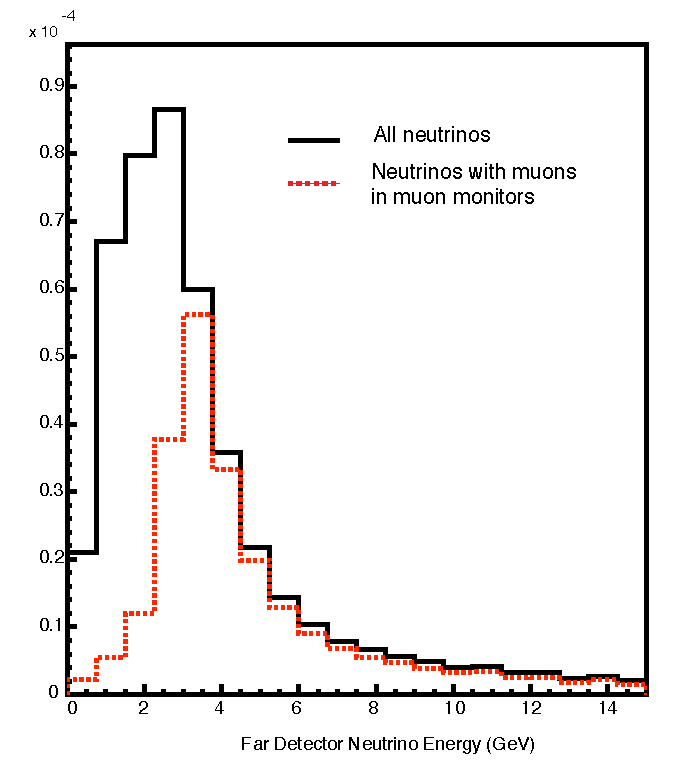
\includegraphics[width=5in,angle=0]{nu_muon_fraction.pdf}
\end{cdrfigure}

\begin{cdrfigure}[Ratio of the flux on-axis to the flux 0.4~mrad off-axis]{fluxRatio}{Ratio of the neutrino flux on-axis to the flux 0.4 mrad off-axis at the Far
Detector position.}
%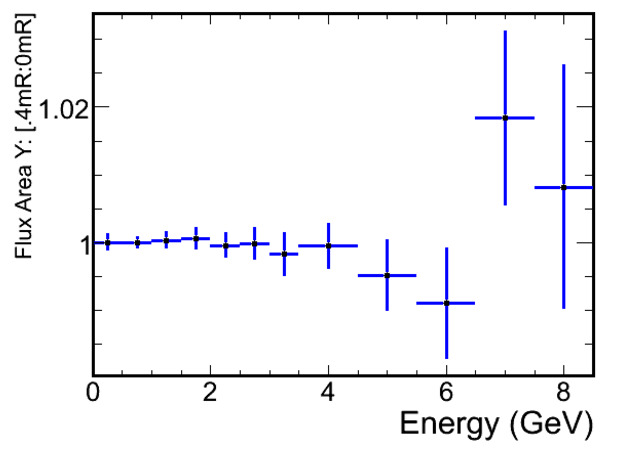
\includegraphics[width=4in,angle=0]{fluxRatio.pdf}
\end{cdrfigure}

It is essential to monitor the stability of the beam direction over
time. Figure~\ref{fig:fluxRatio} shows the effect on the muon-neutrino
flux in the Far Detectors when the beam is misaligned by 0.4~mrad.  
For example, above 6~GeV, the ratio of the Far Detector flux over 
the Near Detector flux changes by 2\%.  
To keep the change in the neutrino beam less than 1\% in all energy bins,
the beam direction must be known to a precision of approximately 0.2~mrad. 
Because the muon monitors will be located approximately 275~m
from the beam target, this requires a measurement of the muons to an
accuracy of approximately 5~cm.


The rate of muons crossing the monitors will be quite high, with
preliminary LBNF beam simulations suggesting approximately 50 million
muons per cm$^{2}$ for a pulse of $10^{14}$ protons-on-target. The
muon monitors must also be capable of operating in a high-radiation
environment.  For example, the expected dose in the area downstream of
the NuMI absorber is as high as 100~MRad per year \cite{ref:NuMIBeamMonitors}.

%
%
%%%%%%%%%%%%%%%%%%%%%%%%%%%%%%%%%%%%%%%%%%%%%%%%%%%%%%%
\section{Muon-Measurement Facilities}
\label{sec:nd-blm-muon-measurement-facilities}

The muon measurements are carried out in the region immediately
following the hadron absorber at the end of the decay tunnel, below
the Absorber Service Building (LBNF 30).  An elevation view
of the absorber area and the muon alcove is shown in Figure~\ref{fig:AbsorberHallElevation}. 
The axis of the decay pipe cuts across the muon alcove at an angle, and the size of the alcove
is largely determined by the requirement that it contain the
shadow of the four-meter-diameter decay pipe, projected through the
alcove, as shown by the blue lines in the elevation view of Figure~\ref{fig:AbsorberHallElevation}. 

Figure~\ref{fig:MuonSystemsOverview} shows the downstream side of the
absorber and a conceptual layout of the muon systems described in various sections of this
chapter.  
The absorber itself is encased in concrete. The first set of
muon-measurement devices, from left to right, is a
set of three variable-pressure gas Cherenkov counters, which are
mounted directly to the rear wall of the absorber. Following that is an ion-chamber array and finally a set of stopped-muon counters which are interspersed between walls of
steel ``blue blocks''.   The blue blocks are there to provide several
depths at which to monitor the stopped muons as they range out in the
material. A second ion-chamber array will also be placed farther downstream within the blue blocks.


\begin{cdrfigure}[The Absorber Hall elevation view]{AbsorberHallElevation}{The Absorber Hall elevation view. The Absorber Service Building (LBNF 30) is on the surface and allows for crane access 
to the Absorber Hall. The muon alcove is directly behind the absorber. }
%\includegraphics[width=8in,angle=0]{ABSORBERHallLongSection.pdf}
\end{cdrfigure}

A perspective view of LBNF 30 is shown in Figure~\ref{fig:AbsorberServiceBuilding}, and a detail of the lower level of Absorber Hall
is given in Figure~\ref{fig:AbsorberFloorLevel}.  The HV, water systems and gas systems for the muon monitors will be located nearby on the lower level.
The readout electronics will be located in racks close to the surface. 

\begin{cdrfigure}[The Absorber Hall with LBNF 30]{AbsorberServiceBuilding}{A perspective view of the Absorber Hall and LBNF 30}
%\includegraphics[width=8in,angle=0]{AbsorberServiceBuilding.pdf}
\end{cdrfigure}

\begin{cdrfigure}[The lower level of the Absorber Hall]{AbsorberFloorLevel}{A perspective view of the 
Absorber Hall lower level}
%\includegraphics[width=5in,angle=0]{AbsorberFloorLevel.pdf}
\end{cdrfigure}

It is important to have precise knowledge of the amount of material muons pass
through before they are registered in the muon systems. The absorber
itself is a complex, heterogeneous assembly of various
materials. 
Figures~\ref{fig:AbsorberDetailElev} and~\ref{fig:AbsorberDetailPlan} show the absorber conceptual design (more detail is available in Volume 2 of this CDR). A hole
in the front side of the absorber, at left, is both surrounded and followed by the
aluminum core of the absorber. The core is then surrounded by steel 
and standard steel ``blue blocks'', 
which are in turn surrounded by concrete.  This
complex geometry must be carefully understood and simulated in order
to make the muon measurements effective. 


\begin{cdrfigure}[Absorber conceptual design, elevation view]{AbsorberDetailElev}{Absorber conceptual design. The figure shows
the elevation view of the absorber at the end of the decay tunnel. The beam direction is shown by
the red arrow. The absorber is constructed of several different materials as shown: aluminum (dark blue), concrete (magenta), and steel (other colors).}
%\includegraphics[width=5in,angle=0]{AbsorberDetailElevation.pdf}
\end{cdrfigure}

\begin{cdrfigure}[Absorber conceptual design, plan view]{AbsorberDetailPlan}{Absorber conceptual design, 
similar to Figure~\ref{fig:AbsorberDetailElev}, that 
shows the plan view of the absorber}
%\includegraphics[width=4in,angle=0]{AbsorberDetailPlan.pdf}

\end{cdrfigure}

Figure~\ref{fig:AbsorberDepthVsRadius} shows the energy lost by a
horizontal muon as it traverses the absorber, as a function of the
horizontal distance from the center. In the central region, out to a
radius of roughly 50~cm, the muons lose roughly 5.6~GeV, so that the
lowest-energy muons leaving the absorber at that point correspond to
neutrino energies of $\sim$ 1.5~GeV. At a radius of roughly 70~cm, the
full thickness of steel causes the muons to lose nearly 10~GeV,
corresponding to neutrino energies of $\sim$ 2.6~GeV. From the
perspective of the muon systems it will be desirable to lower these
thresholds if possible. This might be accomplished by using more
aluminum in the front part of the absorber. Of course the first
concerns must be the containment of the radiation field induced by the
proton beam, and the integrity of the absorber itself. 

\begin{cdrfigure}[Energy loss in absorber]{AbsorberDepthVsRadius}{The absorber's approximate
energy loss versus horizontal radius provides an indication of the variation in 
the depth of the absorber. Muons lose between 6 and 10~GeV depending upon where they cross the absorber.}
%\includegraphics[width=5in,angle=0]{AbsorberDepthVsRadius.pdf}
\end{cdrfigure}

\section{Muon-Ionization Measurements}
\label{sec:nd-blm-muon-ionization}

\subsection{Introduction}

Post-absorber muon measurements in most of the recent neutrino-beam
experiments have typically employed a planar array of ionization
counters to measure the muon profile and intensity. The 
NuMI beamline~\cite{ref:NuMIBeamMonitors} and the K2K~\cite{ref:K2K}~\cite{ref:Maruyama}
and T2K~\cite{ref:T2KMuIon}~\cite{ref:T2KMuMon} experiments have all
utilized parallel-plate ionization chambers. These counters have been
shown to work in the high-radiation environment. 

K2K and T2K have also
deployed solid-state silicon detectors~\cite{ref:Maruyama}
\cite{ref:RD42A}. The advantage of silicon is that it is less
sensitive to changes in the air temperature and pressure. However, these %solid-state 
sensors are not as radiation-tolerant as the parallel-plate ionization 
chambers and will only be used in T2K for the initial
beam operation. 

One disadvantage to ionization counters is that they
measure the total ionization deposited from all particle species
(including the delta-ray electrons produced by the muons), making it
challenging to convert the ionization signal into an absolute
muon flux. The DUNE NDC plans to use the ionization counters to monitor
the beam stability, direction and shape, 
but not to determine the
absolute flux of muons or to determine the muon-energy spectrum. Instead, the
stopped-muon counters %(WBS 130.03.03.02) 
and gas Cherenkov detector %(WBS 130.03.03.04)
 will be used, respectively, to determine the flux and energy
spectrum of the muons. 

\subsection{Reference Design}

The conceptual design for the DUNE muon-ionization chambers is similar
to that used in NuMI, K2K and T2K.  Due to their high radiation
tolerance, sealed ionization counters are the default technology.  For
example, the CERN neutrino beam to Gran Sasso (CNGS) 
system uses an array of Large Hadron Collider (LHC) 
 beam-loss monitors. For DUNE, it might be desirable to investigate solid-state devices
besides silicon, such as diamond detectors (which are approximately an
order of magnitude more radiation-tolerant than silicon counters
\cite{ref:RD42A}\cite{ref:K2KMuDecayMon} ), to deploy as a cross-check of the gas
ionization counters.

Figures \ref{fig:IonChamberLayout} and \ref{fig:IonChamberHousing}
show the conceptual design for the ion-chamber array. Our conceptual
design is based on commercial ion chambers made by LND, Inc. (model 50343). 
%\fixme{use a ref instead, put URL there, later...}
%(http://www.lndinc.com) 
%to base the system on. 
This chamber operates at 400~V and is designed to be sensitive to muons and insensitive to 
backgrounds such as neutrons. 
Radiation-hardened cables will be used to carry the signal to waveform
digitizers, providing a complete spill-by-spill record of the
muon beam.

\begin{cdrfigure}[Model of ion chamber layout]{IonChamberLayout}{A model of the ion chamber layout on the back wall of the absorber
showing the $7\times 7$ grid configuration and supporting Unistrut rails.}
%\includegraphics[width=3in,angle=0]{IonChamberLayout.pdf}

\end{cdrfigure}

\begin{cdrfigure}[Model of ion chamber housing]{IonChamberHousing}{A model of the ion chamber housing and a section showing the commercial ion chamber inside the housing}
%\includegraphics[width=3in,angle=0]{IonChamberHousing.pdf}
%\includegraphics[width=3in,angle=0]{IonChamberSection.pdf}
\end{cdrfigure}

The reference design for DUNE includes two layers of ionization counters, one 
behind the absorber and a second one behind steel shielding blocks. The chambers
will be mounted in a $7 \times 7$ grid (with some missing elements), approximately two meters by two meters. 
DUNE wants to achieve a precision in the beam center of 0.2~milliradians
(5~cm for a 250~m decay pipe). A quick study has 
determined the optimal arrangement of 25 ionization counters for each layer. 
For comparison, the NuMI monitor planes consist of a 
9 $\times$ 9 array, and the T2K monitors use a 7 $\times$ 7 array of counters. 
The decision to use 25 counters for DUNE was motivated by a desire to see if a 7x7 array with some of the diagonal counters removed could achieve the desired sensitivity, thus reducing the total number of needed counters.

\begin{cdrfigure}[Ion chamber performance for grid layout]{ion_grid}{On the left: Precision as a function of detector width for a grid 
shaped detector with 5\% random calibration offsets. On the right: The 
arrangement of ionization counters for the ``5 by 5 grid'' layout.}
%\includegraphics[width=70mm]{grid.pdf}
%\includegraphics[width=50mm]{gridlayout.pdf}
\end{cdrfigure}

\begin{cdrfigure}[Ion chamber performance for cross-with-corners layout]{cross_grid}{On the left: Precision as a function of detector width for a cross-shaped detector 
with 5\% random calibration offsets. On the right: The 
arrangement of ionization counters for the ``cross with corners'' layout.}
%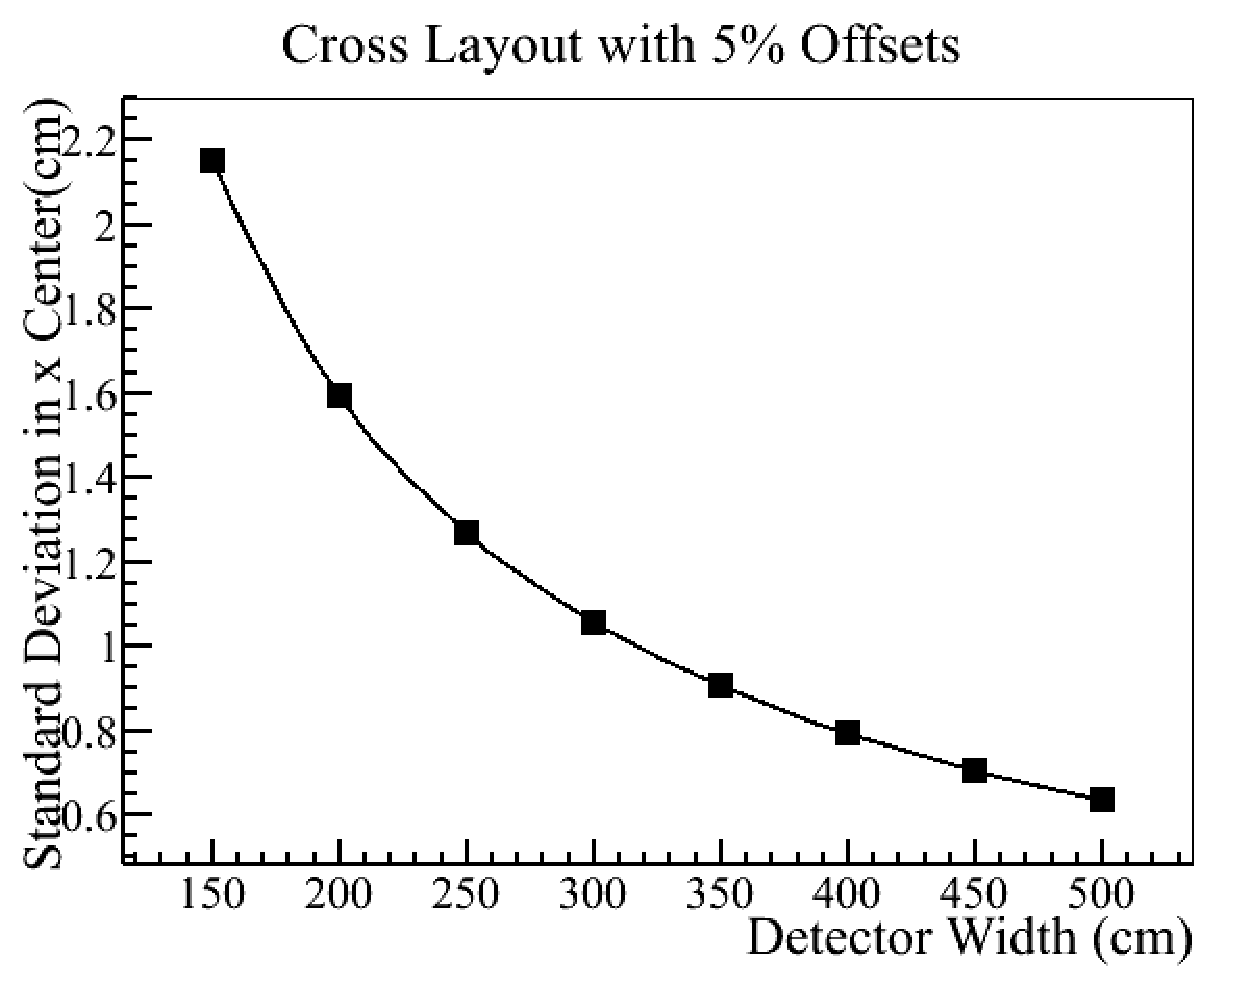
\includegraphics[width=70mm]{cross.pdf}
%\includegraphics[width=50mm]{crosslayout.pdf}
\end{cdrfigure}

Several different designs for the counter arrangement were studied and the
area covered by the detectors was varied. A toy Monte Carlo model was
developed to estimate the precision of each design. The muon profile
was assumed to be a Gaussian with a spread of 130~cm in the $x$ and $y$
dimensions and a center at the origin. 
The standard deviation on the beam center was studied as a
function of array coverage for several designs and for 2\%, 5\% and
10\% random systematic error offsets. Figure~\ref{fig:ion_grid} shows the
precision of the detector array as a function of the width of the
detector for a grid design and with 5\%
offsets. Figure~\ref{fig:cross_grid} shows the same plot for a
``cross with corners'' layout.



The results show that the width of the detector array affects the
precision more than the layout of the detectors. Increasing the array
size improves the precision greatly. Concentrating the ionization
counters to the outside of the layout gave the best precision for this
simple model, but only by a small amount. Even for the layouts with
10\% offsets and a width of 150~cm, the standard deviation on the beam
center was less than our goal of 5~cm.

The DUNE muon ionization chamber design consists of two arrays of 
ionization counters, which is motivated by the NuMI target experience.  As shown in Figure~\ref{fig:numi_target_decay}, over a period of several months, the number of events per proton on target gradually decreased over time, especially in the energy range from 2-4 GeV.  
This reduction in neutrino flux is attributed to 
target radiation damage.  Figure~\ref{fig:numi_mumon_ratio} shows the ratio of the signal seen  in the first muon alcove to the signal seen in the second muon alcove versus time.  This ratio decreased in a similar manner over time.  
The first alcove was immediately after the absorber, while the second alcove was behind approximately 12 m of rock, and therefore saw only higher energy muons, since the lower energy ones would range out before reaching the second alcove.  
This gradual decrease in the ratio of the signals seen in these arrays was an indication of the target degradation and the relative reduction in the 
low-energy part of the neutrino and muon fluxes.  \footnote{Similar trends were seen in the ratios of the other muon alcove signals, but the first/second ratio saw the largest effect.}

It will be necessary to be able to monitor this ratio in DUNE on a spill-by-spill basis to look for signs of target degradation or horn failure.  
Therefore, a second ionization array, placed behind several layers of 
shielding blocks, will be necessary.  In Figure~\ref{fig:MuonSystemsOverview}
the second array is placed behind 4 m of steel shielding.  Since the density of steel is roughly 3 times larger than that of rock, this is comparable to the depth of the NuMI second muon alcove, which sits behind 12 m of rock.  More detailed studies will need to be performed to determine if this is the optimal location for sensitivity to changes in the target density.


\begin{cdrfigure}[NuMI target experience]{numi_target_decay}{Shown here is the number of events observed in the MINOS near detector per proton on target.  The horizontal axis is divided into energy bins.  The gray line shows the average number of events in each energy slice over the whole time period.  Within each energy bin each cross indicates the value in roughly one month of running, with time increasing to the right.}
%\includegraphics[width=5in]{NuMITargetExperience.pdf}
\end{cdrfigure}


\begin{cdrfigure}[NuMI muon monitor ratios]{numi_mumon_ratio}{lShown here is the ratio of the signal seen in 
the NuMI first muon alcove over the signal seen in the second muon alcove over time.  The step that occurs on approximately  December 31, 2006 is when the NuMI decay volume was changed from vacuum to helium, and this change is expected to attenuate the higher energy muon flux more than the lower energy flux.}
%\includegraphics[width=5in]{numi_mm1mm2_ratio.pdf}
\end{cdrfigure}

\subsection{Prototype Design and Testing}

For the gas ionization detectors, a small array of prototype
counters will be built and operated in the existing NuMI
alcoves to determine the optimal design and operating conditions for
the DUNE monitors. This will be done during the long
shutdown for the NOvA upgrade that will end in Spring 2013. 
It will provide a good field test in roughly the same environment as expected during DUNE
operations. It will also be cross-checked against the existing NuMI
muon-monitoring system.  The goals of these tests are to understand the linearity of the response of these counters (by comparing the observed signal to variations in the beam intensity), their long-term stability and operational reliability.  

\subsection{Installation}

The system installation will begin following completion of the
Absorber Hall and LBNF 30
and the installation of the stopped-muon counter system
(described in Section~\ref{sec:nd-blm-stopped-mu}).

\subsection{Operation}

The muon-monitor-system data will be displayed in the control room 
at the Absorber Hall upper level on
a spill-by-spill basis to monitor the beam stability and look for potential signs of target or horn degradation. 
This control room will be accessible during the beam operation.
The data will also be displayed at central run control.  

%
%
%%%%%%%%%%%%%%%%%%%%%%%%%%%%%%%%%%%%%%%%%%%%%%%%%%%%%%%
\section{Stopped-Muon Detector} % (WBS 130.03.03.02)}
\label{sec:nd-blm-stopped-mu}

\subsection{Introduction}

The second system under development is stopped-muon counters, also called
Michel-electron detectors. This method will measure the muon flux without
suffering from some of the disadvantages intrinsic to systems that
detect through-going muons. The strategy employed here is to stop muons
in a material with significant carbon content 
and, via muon capture, to produce $^{12}B$ that will in turn undergo $\beta$ decay.
 The high-carbon material, in this case graphite, surrounds a Cherenkov radiator
material which is sensitive to electrons from muon decay or 
high-energy beta decays.  Figure~\ref{fig:MichelDecayOptions} shows the conceptual design 
of a 
single stopped-muon counter. 


\begin{cdrfigure}[Michel-electron detector conceptualization]{MichelDecayOptions}{Conceptual design of a single Michel-electron detector (stopped-muon counter)}
%\includegraphics[width=5in,angle=0]{StoppedMuonCounter.pdf}
\end{cdrfigure}

The detectors will only operate in the lower-rate
environment that is present many microseconds after the beam pulse is
over. There are two possible modes for this type of system. 
The first is an integrating mode where the characteristic decay time of 
2.2~$\mu s$ for muon decay and corresponding beta-decay lifetimes is used to
unfold the total number of decays. The other mode under
investigation uses the ability to record individual decays rather
than an analog current measurement. This mode may allow a more precise absolute
normalization of the flux and fit the muon lifetime in the Michel-electron detector. 
This will provide a more robust cross-check on the
muon signal than will ionization detectors, which are sensitive to delta
rays, photon conversions and other charged particles.

Although this technique has never been tried on a large scale, a small
demonstration project in K2K was able to see Michel decays with a
$10^{3}$ signal/background ratio and to measure the absolute rate with
30\% precision\cite{ref:K2KMuDecayMon}.

\subsection{Reference Design}

The stopped-muon detector reference design
is modular and based on a Cherenkov radiator of
minimum size to contain a 52.8-MeV electron and distinguish it cleanly
from lower-energy radioactivity. This conceptual design employs
a liquid H$_2$O radiator, although mineral oil and aerogel are other
possible radiator materials. The radiator will be coupled to a photomultiplier tube (PMT) or
other photon counter. Graphite has been chosen for the material
surrounding the radiator as it provides the $^{12}C$ necessary for
producing $^{12}B$ via muon capture. The entire module will be
encased in a material that provides both a uniform-density stopping
target for muons and some shielding from incoming neutrons. One or two
signal channels will be associated with each module, and the full
waveform from each channel over approximately 100~ms will be recorded
on each beam pulse.

Nine modules will be placed just behind the absorber in a cross pattern.  An additional 12 will be 
placed at multiple depths in the
shielding in order to sample the muon flux
from different energies, as shown in Figures~\ref{fig:MuonSystemsOverview} and \ref{fig:StoppedMuonLayout}. 
The shielding will simultaneously act to range out the muons and shield the detectors from 
neutrons. The Cherenkov light from Michel-decay electrons will exit the 
counter and be collected by either nearby PMTs or by a light guide which will
guide the light to a remote optical sensor.  

To probe the muon flux at lower energies, it may also
be feasible and/or desirable to place some additional modules within
the downstream part of the absorber or in the outermost radii of the
decay-pipe shielding. The ability to do this may be limited, however,
by the presence of muons from stopped, positively charged pion decays
due to nearby hadron showers.


\begin{cdrfigure}[Arrangement of blue blocks and Michel-decay detectors]{StoppedMuonLayout}{A top view of the 
lower level of the Absorber Hall showing a possible arrangement of ``blue blocks'' 
and Michel-decay detectors. In this case there is roughly 2~GeV of energy loss 
per wall of blue blocks. The counters can be moved between layers and within a single layer.}
%\includegraphics[width=5in,angle=0]{StoppedMuonLayout.pdf}
\end{cdrfigure}

Besides the Michel decays of stopped muons, the system will
independently measure both the $\mu ^{+}$ and $\mu ^{-}$ stopped
rates as a function of depth. 
While the 2.2~$\mu $s decay time of the $\mu^+$ is a reliable
signature, in graphite roughly 8.5\% of the $\mu^{-}$ undergo capture
on the $^{12}C$ nucleus, and 15\% of those leave behind a $^{12}B$
ground state nucleus. That $^{12}B$ nucleus will undergo $\beta$ decay
with a half-life of 20.20~ms and an electron spectrum with an endpoint
of 13~MeV. With a graphite layer around the detector, this signal is
expected to yield a reliable measurement of the rate of stopped
$\mu^{-}$.

\subsection{Prototype Development and Testing}

Prototype development activity for the Michel-electron detectors will
be divided into studies of the rate and radiation environment where
the detectors will be located and development of the counters
themselves.

The radiation environment will be studied both with Monte Carlo 
simulations and by
measurements from initial prototype detectors in the NuMI muon alcoves
\cite{ref:NuMIBeamMonitors}.
Studies will be performed to determine if the photon sensors
can survive the radiation environment at the location of the Michel
detector. If the sensors can survive, they can be attached directly to
the Cherenkov medium; if not, optical guides will have to bring the
light to a lower-radiation area to the side of the beam. Potential
radiation damage to the Cherenkov radiator itself will also be
studied.

The detector design will focus on selecting radiator and shielding
material, photon-detection technology and control/readout
hardware. Possible radiators include aerogel, which may be designed to
be replaced periodically, and flowing liquids such as H$_2$O or
mineral oil. Long-timescale saturation from the very high-rate
environment of the beam spill could affect the photon-counting devices
\cite{ref:HighRateCounting}. Thus, it will likely be necessary to
design fast-switching, high-voltage circuits that turn on the photon
counters in the first few microseconds after the spill is over. A
similar system was developed in the 1990s for the Brookhaven Muon
(g-2) Experiment~\cite{ref:G2} .

\subsection{Installation}

The stopped-muon counters will be installed after completion of the 
Absorber Hall and LBNF 30  
and installation of the absorber. 
They will be placed into the spaces between the blue-block walls on
support frames.   There will be access to the areas between the shield blocks 
from the side, and the stopped-muon counters will be designed so that they can 
be wheeled in from the side.  If needed, they could then be moved around to measure
the stopped-muon rates across the muon beam.

\subsection{Operation}

The muon-monitor-system data will be displayed in the control room on
a spill-by-spill basis to monitor the beam stability. Because the
system will be located in a radiation-controlled environment that will
not be accessible during the beam operation, it is essential that the
electronics be designed for remote operation.

%
%
%%%%%%%%%%%%%%%%%%%%%%%%%%%%%%%%%%%%%%%%%%%%%%%%%%%%%%%
\section{Muon Cherenkov Detectors} % (WBS 130.03.03.04)}
\label{sec:nd-blm-muon-cherenkov}

\subsection{Introduction}

As mentioned in Section~\ref{sec:nd-blm-muon-measurement-facilities}, one disadvantage of an ionization system for the
muon monitors is that it measures the ionization due to all
particles, including delta-ray electrons and neutrons. This makes it
difficult to determine the muon flux.  Furthermore, the ionization
system is unable to measure the momentum distribution of the
muons. To resolve this problem, a Cherenkov
counter will be deployed downstream of the absorber.  A Cherenkov counter deployed by DUNE
will not image individual Cherenkov rings, but rather will see the
integrated signal from many muons due to the very large instantaneous flux. 
In addition, by varying the radiator gas pressure, and hence the Cherenkov threshold, the system's index of refraction will vary, allowing it to map out the muon momentum distribution.


Figure~\ref{fig:MuonBeta} shows the expected distribution of
velocities, $\beta$ ($v/c$), for muons and electrons after exiting the
absorber. 
Figure~\ref{fig:MuonAngle} shows the expected angle with respect to the beam for
electrons and muons with similar velocities (implying that both are visible above the 
same Cherenkov threshold).  Despite the similar velocities, the muons are much more likely
than the electrons to be directed parallel to the beam.

Therefore, a detector that takes advantage of the directional nature of Cherenkov
light will have less background contributions from
electrons 
and other isotropic background particles such as neutrons, than will an ionization system, for example. 

\begin{cdrfigure}[Simulated electron and muon velocities upon exiting absorber]{MuonBeta}{Simulated electron and muon velocities exiting the absorber. This plot is based on a 
simulation gnumi\cite{GNuMI} of the LBNF beamline.}
%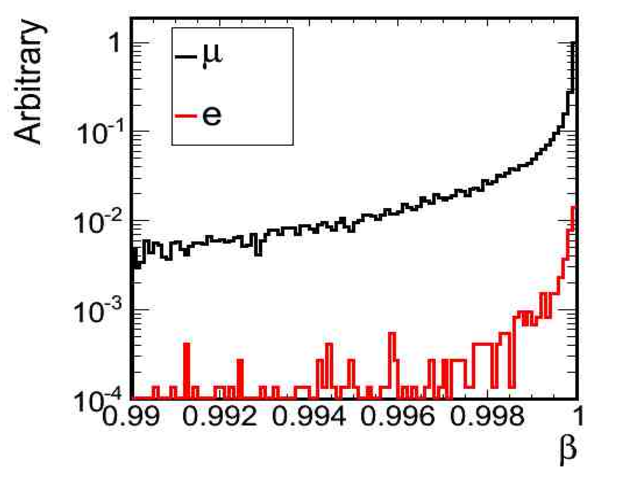
\includegraphics[width=4in,angle=0]{MuonBeta.pdf}
\end{cdrfigure}


\begin{cdrfigure}[Simulated electron and muon angles upon exiting absorber]{MuonAngle}{lSimulated plot of angle with respect to the beam for 
electrons and muons exiting the absorber.
This plot is based on a gnumi simulation of the LBNF beamline.}
%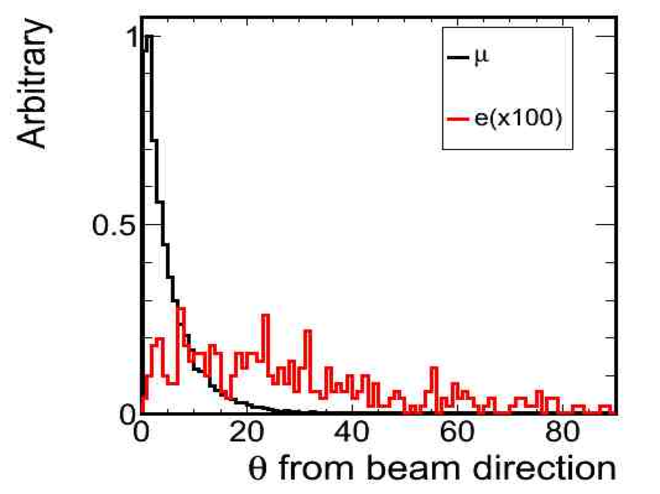
\includegraphics[width=4in,angle=0]{MuonAngle.pdf}
\end{cdrfigure}


\subsection{Reference Design}

There are a number of possible designs for Cherenkov counters. The
conceptual design is based on a traditional beamline Cherenkov
counter, where a gas radiator is contained in a pressurized tube. The
Cherenkov light in a narrow cone is collected at the end of the tube
by a mirror that reflects the light 90 degrees towards a photosensor
located outside the high-radiation field of the alcove. The gas
pressure, varied from vacuum to several atmospheres, will determine
the index of refraction, and hence the muon-momentum
threshold. Several such tubes will be constructed in an array
transverse to the beam direction. The resulting pressure scan will
give the momentum distribution of the muons at an array of points
across the end of the absorber.  

Figure~\ref{fig:CherenkovCounterDetail} shows how the
Cherenkov system will 
be constructed. Safety considerations suggest that the
diameter of the radiator tube and light-guide tube be six inches
or less.  A 
photosensor, located outside the direct radiation field of the muons, will
view the primary mirror through a telescopic optical system.

\begin{cdrfigure}[[Cherenkov counter design]{CherenkovCounterDetail}{The Cherenkov counter conceptual design. 
Muons at threshold momentum emit forward Cherenkov light which is
reflected via two flat mirrors (one at 90 degrees) 
to a PMT located outside of the muon
radiation field.}
%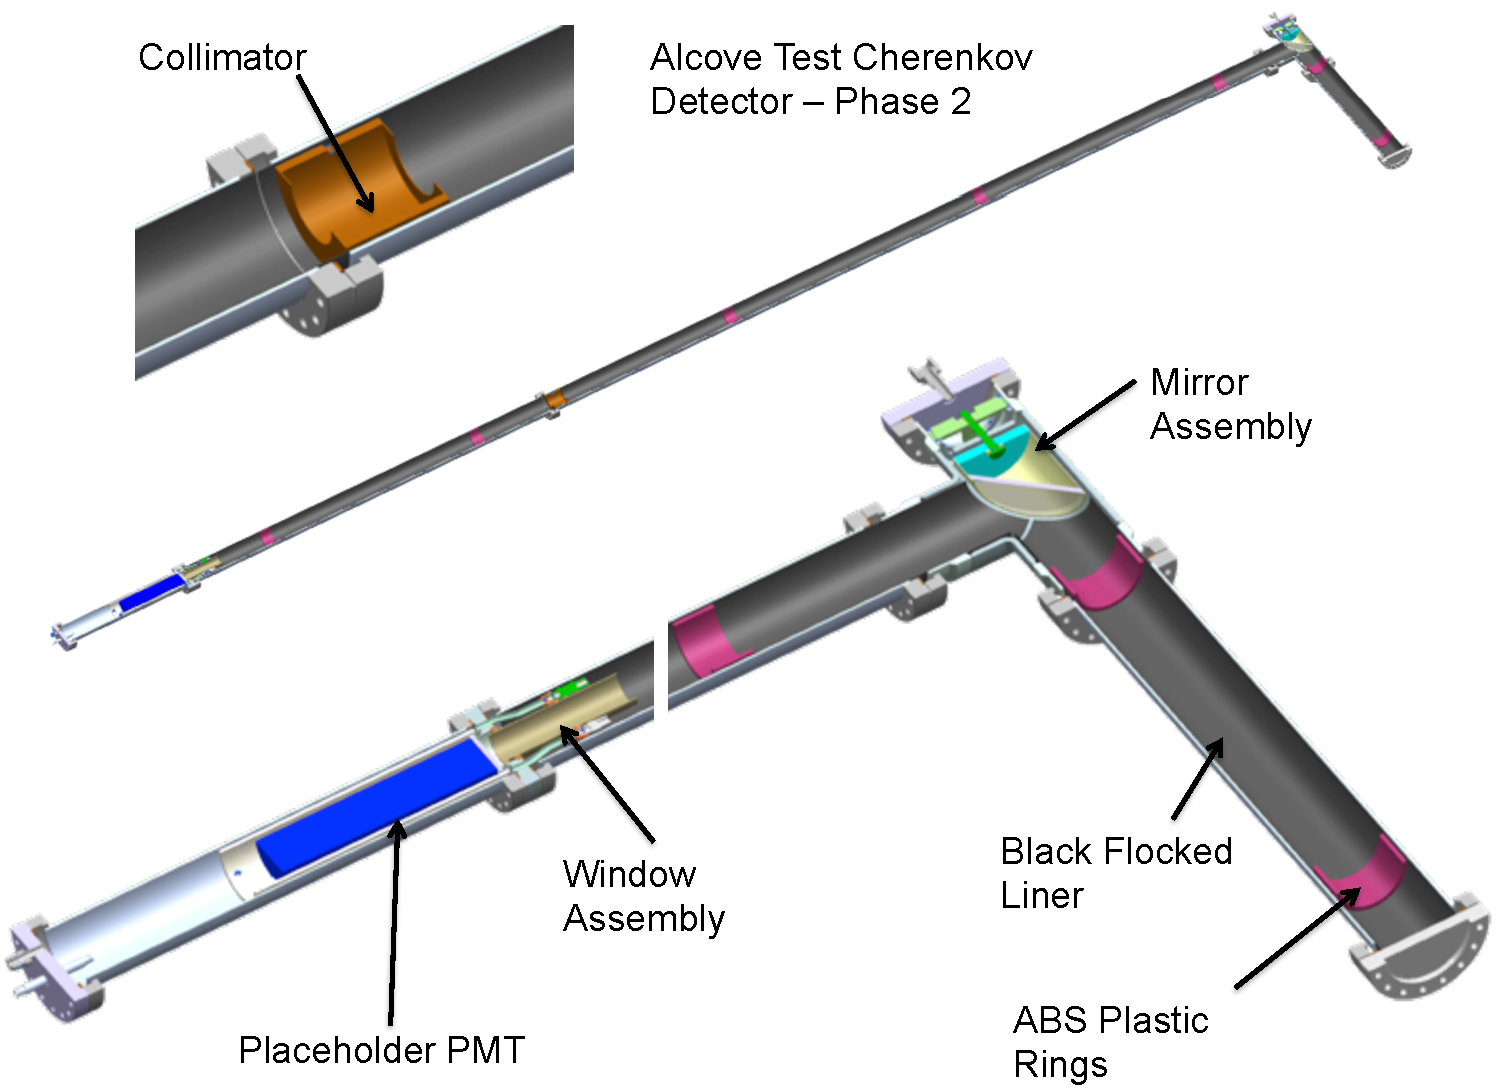
\includegraphics[width=6in,angle=0]{CherenkovCounterDetail.pdf}
\end{cdrfigure}

The layout of the Cherenkov counter system is shown in
Figure~\ref{fig:CherenkovCounterLayout}.

\begin{cdrfigure}[Cherenkov counter layout]{CherenkovCounterLayout}{The layout of one of the muon 
Cherenkov counters behind the rear of the absorber}
%\includegraphics[width=3in,angle=0]{CherenkovCounterLayout.pdf}
\end{cdrfigure}

The preferred option is to use a gas Cherenkov system containing a
noble gas with a high index of refraction, where the density of the
gas can be varied to change the Cherenkov threshold. The noble gas
will reduce potential degradation due to reactivity in the high
radiation field of the post-absorber environment. Varying the pressure
will provide more information about the momentum spectrum of the
muons.

The combination of a flat mirror and a 90$^0$ mirror will reflect
light out to a PMT. The UV-sensitive PMT will collect light from
normal incidence on the primary mirror to $\sim$5~mrad. Figure~\ref{fig:LightYield} 
shows that, with a 5~mrad acceptance, the light
yield per particle will be approximately one photon near
threshold. That is more than ample light for the system where the
particle flux is of order 10$^8$ per cm$^2$ on a PMT. 

One possible background is transition radiation, which occurs when a charged particle moves between materials with different indices of refraction.  This process can generate light in the visible region, and it can occur even when there is a vacuum inside the gas Cherenkov system.
Figure~\ref{fig:LightYield} also shows that the transition radiation
emitted from the mirror surfaces is at least two orders of
magnitude lower than the Cherenkov light yield and thus does not introduce a
significant background.

\begin{cdrfigure}[Cherenkov and Transition Radiation Yields]{LightYield}{The calculated light yields for Cherenkov radiation (left) and transition radiation for muons in argon gas}
%\includegraphics[width=3.2in,angle=0]{CherenkovLightYield.pdf}
%\includegraphics[width=3.2in,angle=0]{TransitionLightYield.pdf}
\end{cdrfigure}

A standalone Geant4~\cite{GEANT4:NIM}  
simulation for a proposed gas Cherenkov detector
for the DUNE muon monitors was developed to investigate various mirror
shapes.  Based on this work, a conceptual design has been developed,
 shown in Figure~\ref{fig:mirrors}.  Here the muons enter on the
right, Cherenkov photons are produced in a region of a dense
gas\footnote{Freon was used in the simulations, but a noble gas is the
prime candidate.}, and the light is bounced off of two mirrors towards a
photosensor that sits in a lower-radiation environment. Based on fits
to a Geant3~\cite{Geant3}  simulation of the muons exiting the absorber, the
following angular distribution was used to describe the probability of
observing a muon with a given angle $\theta$ with respect to the beam axis:
\begin{equation}
Prob(\theta)=A \times \theta e^{\frac{-\theta^2}{2\sigma (p)}}
\end{equation}
where A is an arbitrary normalization and the width, a function of
the momentum $p$, is given by
\begin{equation}
\sigma (p) = 5.903 p^{-0.681}.
\end{equation}
Thus, as the momentum increases, $\sigma (p)$ decreases, and the muons
become more forward-going.

Several different mirror shapes were examined, including spherical and 
conical, but much simpler flat mirrors were found to be adequate. 


\begin{cdrfigure}[Muon gas Cherenkov counter design]{mirrors}{Conceptual design for the muon gas Cherenkov detector for DUNE.  
Muons will travel through an L-shaped pipe filled with a dense gas,
and mirrors will direct the optical photons to a photodetector.}
%\includegraphics[width=3.5in]{cherenkov_layout.pdf}
\end{cdrfigure}

Figure~\ref{fig:varyindex} shows a simulation of 
the number of photons collected at the photosensor versus muon energy for
a range of indices of refraction.  Varying the gas density will allow sensitivity of 
the photon measurements to different parts of the muon-energy spectrum.

\begin{cdrfigure}[Cherenkov counter response to muons]{varyindex}{The number of photons detected in the photosensor vs. muon energy.  
Here 10,000 muons have been simulated at each energy.  The gas density
increases from 0.05~atm in the upper left to 12~atm in the lower
right.}
%\includegraphics[width=6in]{many_indices.pdf}
\end{cdrfigure}

\subsection{Prototype Development and Testing}

Because this type of system has not previously been deployed for a
muon monitor, significant design work and testing will be required. It will
be important to understand the noise and background light from
non-Cherenkov sources, such as fluorescence and scintillation in the
gas and transition radiation. Some of these items will be examined with cosmic muons.  A 
small prototype system will be tested in the NuMI beam alcoves in 2013, where the goals of the testing 
are to understand the linearity of the response and the overall stability of the system, 
including its sensitivity to atmospheric changes such as the ambient temperature and 
pressure, and the long term effects of the radiation.

\subsection{Installation}

Installation
will begin following the installation the stopped muon systems
systems. The gas handling system will be located nearby, also on the 
lower level of the Absorber Hall, as shown in Figure~\ref{fig:AbsorberFloorLevel}.

\subsection{Operation}

Because the system will be located in a radiation-controlled
environment that will not be accessible during beam operation, it is
essential that the electronics and gas handling system be both robust
and remotely operable.  Periodic access may be required to the utilities area to replace gas bottles.
